% Created 2020-08-18 Tue 21:57
% Intended LaTeX compiler: pdflatex

\documentclass[12pt,a4paper]{article}
\usepackage[margin=2cm]{geometry}

\usepackage{hyperref}
\usepackage[utf8]{inputenc}
\usepackage{fixltx2e}
\usepackage{graphicx}
\usepackage{longtable}
\usepackage{float}
\usepackage{wrapfig}
\usepackage{rotating}
\usepackage[normalem]{ulem}
\usepackage{amsmath}
\usepackage{textcomp}
\usepackage{marvosym}
\usepackage{wasysym}
\usepackage{multicol}
\usepackage{amssymb}
\tolerance=1000
\usepackage{listings}
\author{Yung Chin, Yen}
\date{\today}
\title{Basic Materials of C++ Basic}
\begin{document}

\maketitle
\tableofcontents

\newpage

\section{C++基本架構}
\label{sec:orgd5dc298}

\lstset{breaklines=true,language=cpp,label= ,caption= ,captionpos=b,firstnumber=1,numbers=left}
\begin{lstlisting}
#include<iostream>
using namespace std;

int main()
{
    cout << "Hello world\n";
    return 0;
}
\end{lstlisting}

\begin{verbatim}
Hello world
\end{verbatim}


上述程式中,第1行為標頭檔(Header)的引入,這裡告訴 Compiler 說我需要用到 iostream 這個 header,原因是程式的第6行用到 cout 這個指令,而這個指令就被定義在 iostream 這個 header 中,其中的 io 即代表 input/output。\\
\section{Variable}
\label{sec:org768402c}

\lstset{breaklines=true,language=C++,label= ,caption= ,captionpos=b,firstnumber=1,numbers=left}
\begin{lstlisting}
#include <iostream>
using namespace std;
int main() {
    int x;
    x = 32;
    cout << "This is demostration of variable declaration of C++.\n";
    cout << "變數x的內容為: " << x << endl;
}
\end{lstlisting}

\begin{verbatim}
This is demostration of variable declaration of C++.
變數 x 的內容為: 32
\end{verbatim}

\section{if-else}
\label{sec:org4f10f8c}

\subsection{單一條件}
\label{sec:org68d0037}
\lstset{breaklines=true,language=cpp,label= ,caption= ,captionpos=b,firstnumber=1,numbers=left}
\begin{lstlisting}
#include <iostream>
using namespace std;
int main() {
  int x;
  x=31;
  if (x%2==0) {
    cout << "x為偶數\n";
  }
  if (x%2!=0) {
    cout << "x為奇數\n";
  }
}
\end{lstlisting}

\begin{verbatim}
x 為奇數
\end{verbatim}

\subsection{雙重條件}
\label{sec:org548f87f}

\subsection{}
\label{sec:org51e0942}
\lstset{breaklines=true,language=C,label= ,caption= ,captionpos=b,numbers=none}
\begin{lstlisting}
  #include <stdio.h>
  int main() {
      int x=4;
      if (x%2==0) {
         printf("even\n");
      } else {
	     printf("odd\n");
      }
  }
\end{lstlisting}

\section{for}
\label{sec:orgdb7b9ab}

\section{nested for}
\label{sec:org0f31216}

\section{while}
\label{sec:orgacdf5ab}

\section{Instruction to C++}
\label{sec:org3d17a5b}

\section{Variable}
\label{sec:org21cbc94}

\lstset{breaklines=true,language=C++,label= ,caption= ,captionpos=b,firstnumber=1,numbers=left}
\begin{lstlisting}
  #include <iostream>
  using namespace std;
  int main() {
      int x;
      x = 32;
      cout << "This is demostration of variable declaration of C++";
  }

\end{lstlisting}

\section{if-else}
\label{sec:org54a3a2f}

\subsection{單一條件}
\label{sec:orgb2ab9db}
\lstset{breaklines=true,language=C++,label= ,caption= ,captionpos=b,firstnumber=1,numbers=left}
\begin{lstlisting}
  #include <iostream>
  using namespace std;
  int main() {
    int x;
    x=32;
    if (x%2==0) {
      cout << "x為偶數\n";
    }
    if (x%2!=0) {
      cout << "x為奇數\n";
    }
  }
\end{lstlisting}

\subsection{雙重條件}
\label{sec:org7ea0619}

\subsection{}
\label{sec:orgb117875}
\lstset{breaklines=true,language=C,label= ,caption= ,captionpos=b,numbers=none}
\begin{lstlisting}
#include <stdio.h>
#include <iostream>
int x=4;
if (x%2==0) {
  cout << "x為偶數\n";
} else {
  cout << "x為奇數\n";

}
\end{lstlisting}

\section{for}
\label{sec:org2e036f4}

\section{nested for}
\label{sec:org2ca3b8d}

\section{while}
\label{sec:org40c10b9}

\section{function}
\label{sec:org68243c7}

\subsection{function declaration}
\label{sec:org881b470}

\subsection{function define}
\label{sec:org2a330d5}

\subsection{compute n!}
\label{sec:org4fb1fab}
\lstset{breaklines=true,language=C,label= ,caption= ,captionpos=b,numbers=none}
\begin{lstlisting}
  #include <stdio.h>
  int n(int x) {
      if (x==1) {
          return 1;
      } else {
          return x*n(x-1);
      }
  }
  int main() {
      int hi = 5;
      printf("%d\n",n(5));
  }

\end{lstlisting}

\section{function}
\label{sec:org6ffa83d}

\subsection{function declaration}
\label{sec:org4418fb6}

\subsection{function define}
\label{sec:orgc8bc2d3}

\subsection{compute n!}
\label{sec:org22fb942}
\lstset{breaklines=true,language=C++,label= ,caption= ,captionpos=b,numbers=none}
\begin{lstlisting}
  #include <iostream>
  using namespace std;
  int n(int x) {
      if (x==1) {
          return 1;
      } else {
          return x*n(x-1);
      }
  }

  int main() {
      int hi = 9;
      cout << n(8) << endl;
  }

\end{lstlisting}

\section{python}
\label{sec:orgac4d59b}
\lstset{breaklines=true,language=Python,label= ,caption= ,captionpos=b,firstnumber=1,numbers=left}
\begin{lstlisting}
def foo(x):
  if x>0:
    return x+1

  else:
    return x-1

return foo(5)
\end{lstlisting}
\subsection{Python}
\label{sec:orgfe399ab}
\lstset{breaklines=true,language=Python,label= ,caption= ,captionpos=b,firstnumber=1,numbers=left}
\begin{lstlisting}


print "Hello"

\end{lstlisting}

\section{ditaa}
\label{sec:org0194e75}
\begin{center}
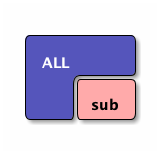
\includegraphics[width=.9\linewidth]{blue.png}
\end{center}
\end{document}
